\chapter{Фурье-двойственность, импульс и движение свободной частицы}

\section{От основ к примерам}

Запутанность занимает центральное место в квантовой механике, но теперь основы изложены достаточно ясно, так что мы можем начать ими пользоваться. До сих пор курс опирался на намеренно малые системы: спин, поворачиваемый прибор, конечный список исходов и повторяющиеся измерения, по которым выводятся вероятности. Эти эксперименты логически проще того исторического пути, которым была открыта квантовая механика, но они содержат минимальный набор операциональных составляющих.

\begin{classroomqa}
\audiencequestion{Что в квантовой механике играет роль небольшого набора эмпирических исходных положений Ньютона?}
\lecturerresponse{Минимальная модель — это поворачиваемый спиновый прибор. Подготовьте спин, выберите ось, нажмите кнопку измерения, запишите \(+1\) или \(-1\) и повторяйте эксперимент, пока не станут известны частоты исходов. Векторное пространство, наблюдаемые, амплитуды и правило Борна организуют эту статистику. Исторически теория возникла из гораздо более богатого набора атомных явлений, но логически этого эксперимента с двумя исходами достаточно, чтобы выявить ее структуру.}
\end{classroomqa}

\begin{classroomqa}
\audiencequestion{Нужно ли проводить одну и ту же статистическую процедуру для каждой физической величины, например спина или импульса?}
\lecturerresponse{Да. Наблюдаемая связана с классом экспериментальных схем и возможных исходов. Формализм предсказывает распределение, как только заданы состояние и наблюдаемая, но физический смысл наблюдаемой закрепляется тем, как ее измеряют.}
\end{classroomqa}

Прежде чем оставить тему запутанности, один вопрос из предыдущего обсуждения заслуживает полного ответа. Рассмотрим два электрона с синглетным и триплетным секторами и включим поле излучения как еще одну квантовую подсистему. Поле излучения имеет вакуумное состояние \(\ket{0_\gamma}\) и однофотонное состояние \(\ket{1_\gamma}\). Само число частиц может находиться в суперпозиции; нет никакого правила, которое ограничивало бы суперпозицию различными состояниями при фиксированном числе частиц.

Для идеализированного перехода, обсуждавшегося на занятии, первоначально незапутанное электронное состояние можно записать как суперпозицию синглетной и триплетной компонент,
\begin{equation}
\ket{\uparrow\downarrow}
=
\frac{1}{\sqrt{2}}
\left(\ket{S}+\ket{T_0}\right).
\end{equation}
Если вначале фотона нет, состояние имеет вид
\begin{equation}
\ket{\Psi(0)}
=
\frac{1}{\sqrt{2}}
\left(\ket{S}+\ket{T_0}\right)
\otimes\ket{0_\gamma}.
\label{eq:l9-initial-radiative-state}
\end{equation}
Синглетная компонента остается синглетной без испускания, тогда как возбужденная триплетная компонента может релаксировать в синглет с испусканием фотона:
\begin{align}
\ket{S}\ket{0_\gamma}
&\longrightarrow
\ket{S}\ket{0_\gamma}, \\
\ket{T_0}\ket{0_\gamma}
&\longrightarrow
\ket{S}\ket{1_\gamma}.
\end{align}
Тогда из линейности следует
\begin{equation}
\ket{\Psi_{\mathrm{final}}}
=
\ket{S}\otimes
\frac{\ket{0_\gamma}+\ket{1_\gamma}}{\sqrt{2}}.
\label{eq:l9-final-radiative-state}
\end{equation}

\begin{figure}[htbp]
\centering
\includegraphics[width=0.88\textwidth]{lecture_09_figure_01.png}
\caption{Электронное состояние разлагается на синглетную и триплетную компоненты и до радиационной релаксации образует тензорное произведение с фотонным вакуумом.}
\lectureframe{00:05:10}
\end{figure}

Последнее выражение является произведением состояний электронной пары и поля излучения. Два электрона запутаны друг с другом, поскольку состояние \(\ket{S}\) является запутанным, тогда как поле излучения остается в суперпозиции нуля и одного фотона. Этот пример тонок, потому что взаимодействие перераспределило запутанность: начальное факторизованное электронное состояние эволюционирует в запутанную электронную пару, однако конечное идеализированное состояние электронов и излучения факторизуется.

\begin{classroomqa}
\audiencequestion{Может ли любой входящий фотон обратить переход и устранить запутанность между электронами?}
\lecturerresponse{Нет. Для процесса, обращенного во времени, требуются соответствующие состояние фотона, мода, фаза, энергия и история взаимодействия. Фраза о том, чтобы отразить испущенный фотон обратно, была сокращенным способом сказать, что нужно организовать обратную эволюцию всей замкнутой системы, а не утверждением, будто произвольный фотон снимет запутанность.}
\end{classroomqa}

\begin{classroomqa}
\audiencequestion{Что заставляет триплет испускать излучение, если не введено никакого внешнего магнитного поля?}
\lecturerresponse{Электроны взаимодействуют друг с другом и с квантованным электромагнитным полем. Их спин-зависимое взаимодействие делает одну спиновую конфигурацию энергетически более выгодной, и избыток энергии может уйти в виде излучения. Никакой внешний измерительный прибор не нужен; это обычная унитарная динамика объединенной системы электронов и поля.}
\end{classroomqa}

Разобравшись с этим оставшимся вопросом, теперь оставим в стороне спин и изучим простейшую задачу о движении: одну частицу на одномерной прямой.

\section{Плоские волны и пара Фурье}

Прежде чем вернуться к физике, нам нужно небольшое математическое отступление. Начнем с
\begin{equation}
e^{ipx}=\cos(px)+i\sin(px).
\end{equation}
На этом этапе \(p\) — просто вещественное число, задающее скорость осцилляции. Это выражение не зависит от времени и потому пока еще не описывает движущуюся волну. Оно называется плоской волной, потому что как функция \(x\) имеет привычную синусоидальную форму.

Широкий класс достаточно регулярных функций можно разложить по таким модам. Мы ограничимся функциями, которые ведут себя достаточно хорошо, чтобы нижеследующие интегралы имели смысл: они не должны расходиться на пространственной бесконечности, а физические волновые функции, которые появятся позже, будут квадратично интегрируемыми. При симметричном соглашении о нормировке пара Фурье имеет вид
\begin{align}
\psi(x)
&=
\int_{-\infty}^{\infty}
\frac{dp}{\sqrt{2\pi}}\,
\widetilde{\psi}(p)e^{ipx},
\label{eq:l9-fourier-forward}\\
\widetilde{\psi}(p)
&=
\int_{-\infty}^{\infty}
\frac{dx}{\sqrt{2\pi}}\,
\psi(x)e^{-ipx}.
\label{eq:l9-fourier-inverse}
\end{align}
Коэффициент \(\widetilde{\psi}(p)\) — это комплексная амплитуда моды с меткой Фурье \(p\). Множители \(1/\sqrt{2\pi}\) условны; если поставить по одному в каждом преобразовании, обе формулы выглядят взаимно-обратными. Относительный знак минус в показателе экспоненты существенен.

\begin{figure}[htbp]
\centering
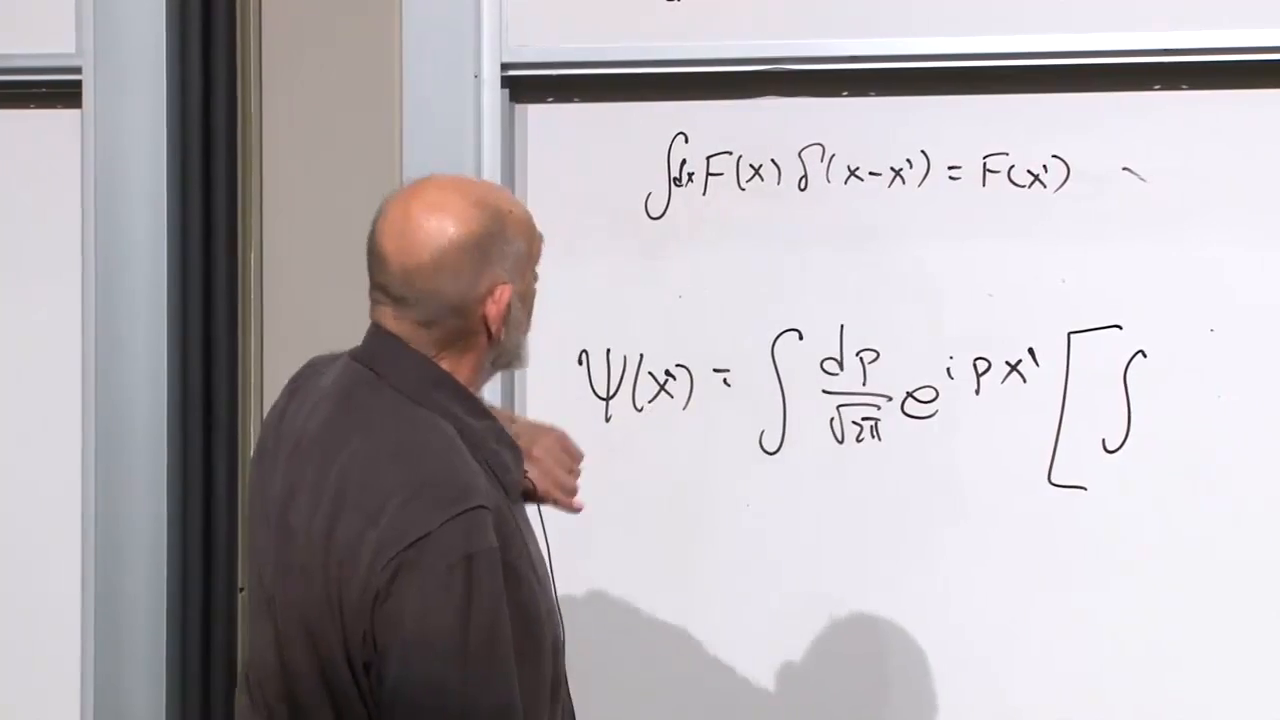
\includegraphics[width=0.88\textwidth]{lecture_09_figure_02.png}
\caption{Симметричная пара Фурье: функция разлагается по плоским волнам, а амплитуды мод восстанавливаются обратным преобразованием.}
\lectureframe{00:14:35}
\end{figure}

\begin{classroomqa}
\audiencequestion{Предполагается ли, что \(\psi(x)\) и \(\widetilde{\psi}(p)\) являются комплексными?}
\lecturerresponse{Вообще говоря, да. В частном случае функция может оказаться вещественной; тогда ее коэффициенты Фурье удовлетворяют дополнительному соотношению сопряжения, но квантовые амплитуды естественно комплексны, и здесь никакого ограничения на вещественность не вводится.}
\end{classroomqa}

\begin{classroomqa}
\audiencequestion{Почему используются симметричные множители \(1/\sqrt{2\pi}\), а не помещается весь \(2\pi\) в одно из преобразований?}
\lecturerresponse{Оба соглашения согласованы. Симметричный выбор делает прямое и обратное преобразования различающимися только знаком в экспоненте. Физические предсказания не зависят от соглашения, если все связанные нормировки изменяются согласованно.}
\end{classroomqa}

Взаимная связь между \(x\) и \(p\) уже видна. Одна функция представляется интегрированием по другой переменной. Пока это просто анализ Фурье. Скоро эта же пара станет координатой и импульсом.

\section{Дельта-функция Дирака как операция}

Интуитивно дельта-функция — это пик исчезающей ширины, бесконечной высоты и единичной площади. Эта картина полезна, но операционное определение надежнее. Для всякой подходящей пробной функции \(f\),
\begin{equation}
\int_{-\infty}^{\infty}
dx\,\delta(x-x')f(x)
=f(x').
\label{eq:l9-delta-sampling}
\end{equation}
Ту же идею выражают три знакомых правила:
\begin{align}
f(x)\delta(x-x')
&=
f(x')\delta(x-x'),
\label{eq:l9-delta-multiplication}\\
\int_{-\infty}^{\infty}dx\,\delta(x-x')
&=1,
\label{eq:l9-delta-area}\\
\int_{-\infty}^{\infty}dx\,\delta(x-x')f(x)
&=f(x').
\end{align}
Первое правило верно, потому что дельта-функция имеет носитель только там, где \(x=x'\). Во втором правиле сдвиг пика меняет его положение, но не его площадь. Объединяя эти два правила, получаем третье.

\begin{figure}[htbp]
\centering
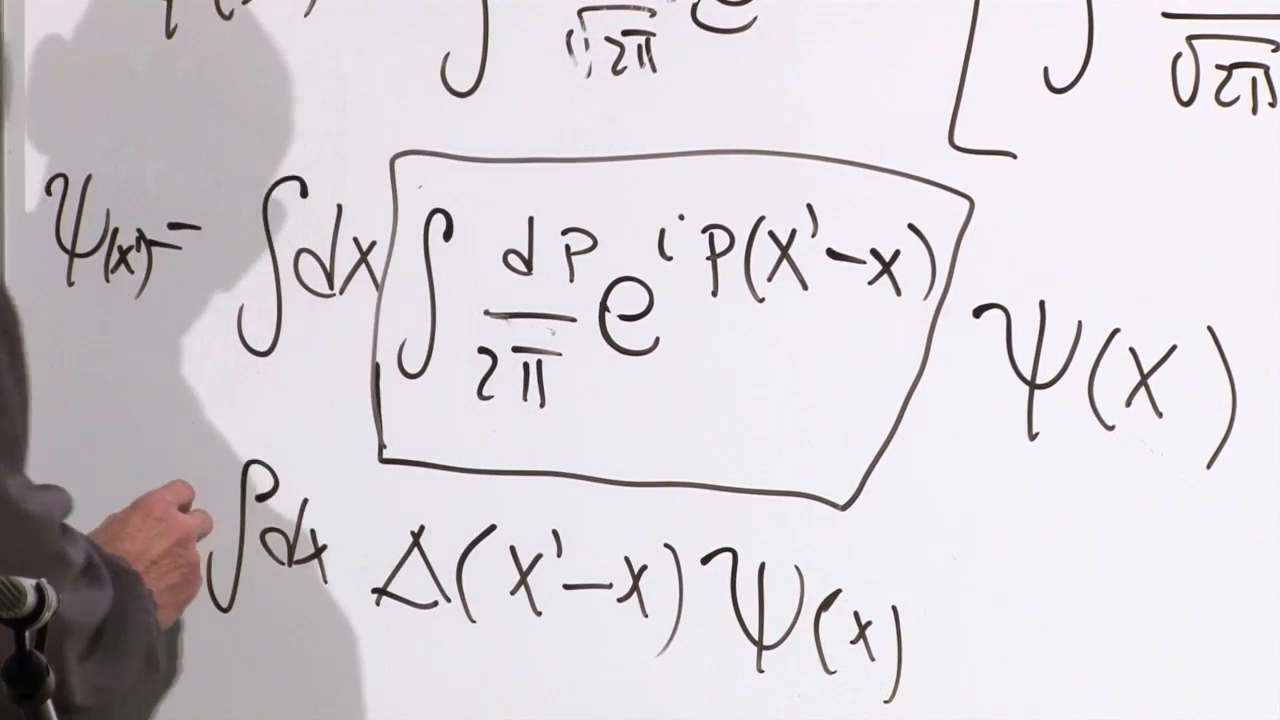
\includegraphics[width=0.88\textwidth]{lecture_09_figure_03.png}
\caption{Свойство выборки, которое характеризует дельта-функцию Дирака по ее действию на всякую подходящую функцию.}
\lectureframe{00:19:45}
\end{figure}

\begin{classroomqa}
\audiencequestion{Почему \(f(x')\) можно вынести за знак интеграла по \(x\)?}
\lecturerresponse{Переменная интегрирования — \(x\). Метка \(x'\) фиксирована при этом интегрировании, так что \(f(x')\) есть константа по отношению к \(x\). Оставшийся интеграл от дельта-функции имеет единичную площадь.}
\end{classroomqa}

Дельта-функция не является обычной поточечно определенной функцией. В частности, попытка возвести ее в квадрат приводит к объекту, более сингулярному, чем исходная дельта-функция. Ее корректный смысл — в смысле распределений: уравнение~\eqref{eq:l9-delta-sampling} задает ее действие под знаком интеграла.

\subsection{Фурье-представление дельта-функции}

Подставим уравнение~\eqref{eq:l9-fourier-inverse} в уравнение~\eqref{eq:l9-fourier-forward}, переобозначив аргумент слева как \(x'\):
\begin{align}
\psi(x')
&=
\int\frac{dp}{\sqrt{2\pi}}\,
e^{ipx'}
\left[
\int\frac{dx}{\sqrt{2\pi}}\,
\psi(x)e^{-ipx}
\right] \notag\\
&=
\int dx
\left[
\int\frac{dp}{2\pi}
e^{ip(x'-x)}
\right]\psi(x).
\label{eq:l9-fourier-composition}
\end{align}
Выражение в квадратных скобках должно воспроизводить \(\psi(x')\) для всякой подходящей функции \(\psi\). Сравнение с определяющим действием дельта-функции дает
\begin{equation}
\boxed{
\int_{-\infty}^{\infty}
\frac{dp}{2\pi}\,
e^{ip(x'-x)}
=\delta(x'-x)
}.
\label{eq:l9-delta-fourier-x}
\end{equation}

\begin{figure}[htbp]
\centering
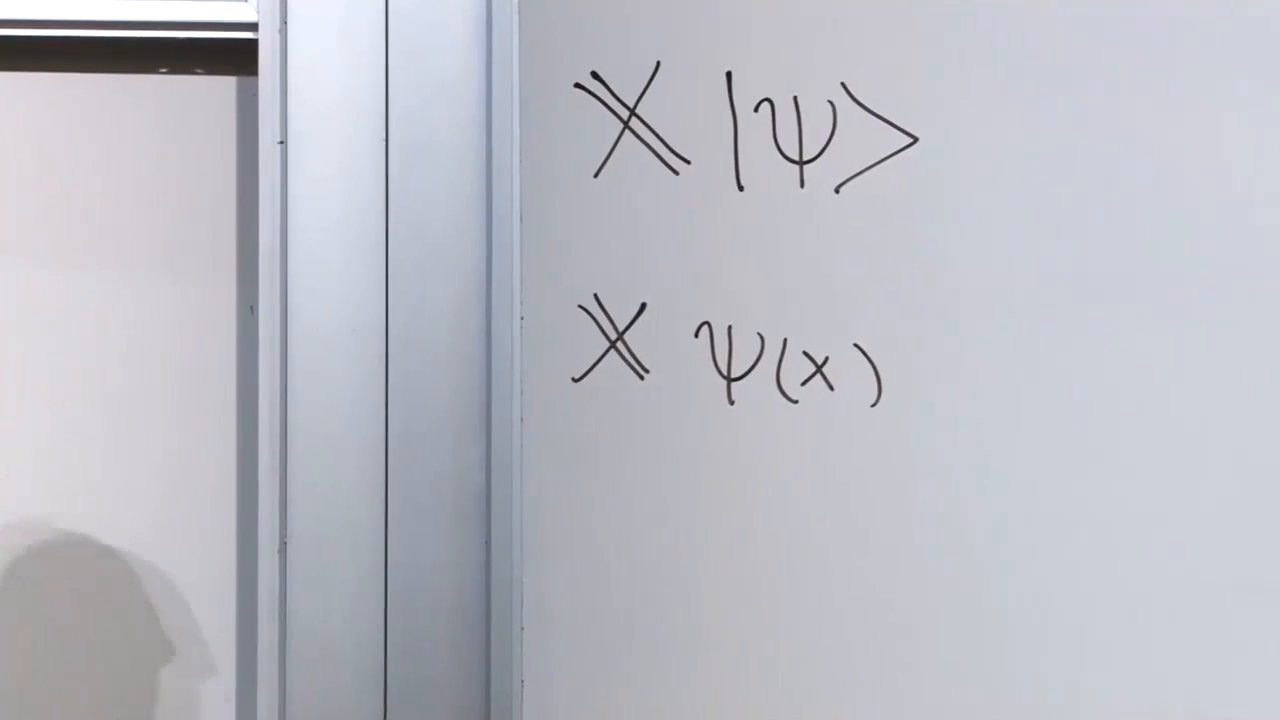
\includegraphics[width=0.88\textwidth]{lecture_09_figure_04.png}
\caption{Ядро Фурье выделяется внутри композиции двух преобразований и по своему выборочному действию отождествляется с дельта-функцией Дирака.}
\lectureframe{00:26:23}
\end{figure}

Если поменять местами названия взаимно-двойственных переменных, получается сопутствующее тождество
\begin{equation}
\boxed{
\int_{-\infty}^{\infty}
\frac{dx}{2\pi}\,
e^{ix(p-p')}
=\delta(p-p')
}.
\label{eq:l9-delta-fourier-p}
\end{equation}
Тем самым дельта-функция является непрерывной суперпозицией плоских волн.

\begin{classroomqa}
\audiencequestion{Один раз показатель экспоненты был записан как \(x'-x\), а в другом месте как \(x-x'\). Меняет ли смена знака результат?}
\lecturerresponse{Нет. Дельта-функция четна: \(\delta(u)=\delta(-u)\). Поэтому изменение знака разности не меняет конечного распределения. Промежуточный экспоненциальный множитель переходит в свой комплексно-сопряженный вид, но проинтегрированное ядро остается той же дельта-функцией.}
\end{classroomqa}

В этих выкладках опущена оговорка о сходимости. Осциллирующие интегралы — это распределения, а не абсолютно сходящиеся обычные интегралы, и перестановка порядка интегрирования требует осторожности. Удобную регуляризацию даёт конечный периодический интервал: сначала используются дискретные моды Фурье и кронекеровская ортогональность, затем длину интервала устремляют к бесконечности. Приведённые выше тождества непрерывного случая и есть возникающий в результате предел.

\section{Частица на прямой}

Классически состояние задаётся одной точкой в фазовом пространстве:
\begin{equation}
(x,p).
\end{equation}
Квантовая механика начинает с другого вопроса: какой ортонормированный базис определяет пространство состояний? Для каждого вещественного положения \(x\) введём обобщённый собственный кет \(\ket{x}\). Произвольное состояние можно разложить как
\begin{equation}
\ket{\Psi}
=
\int_{-\infty}^{\infty}
dx\,\psi(x)\ket{x},
\qquad
\psi(x)=\braket{x}{\Psi}.
\label{eq:l9-position-expansion}
\end{equation}

\begin{figure}[htbp]
\centering
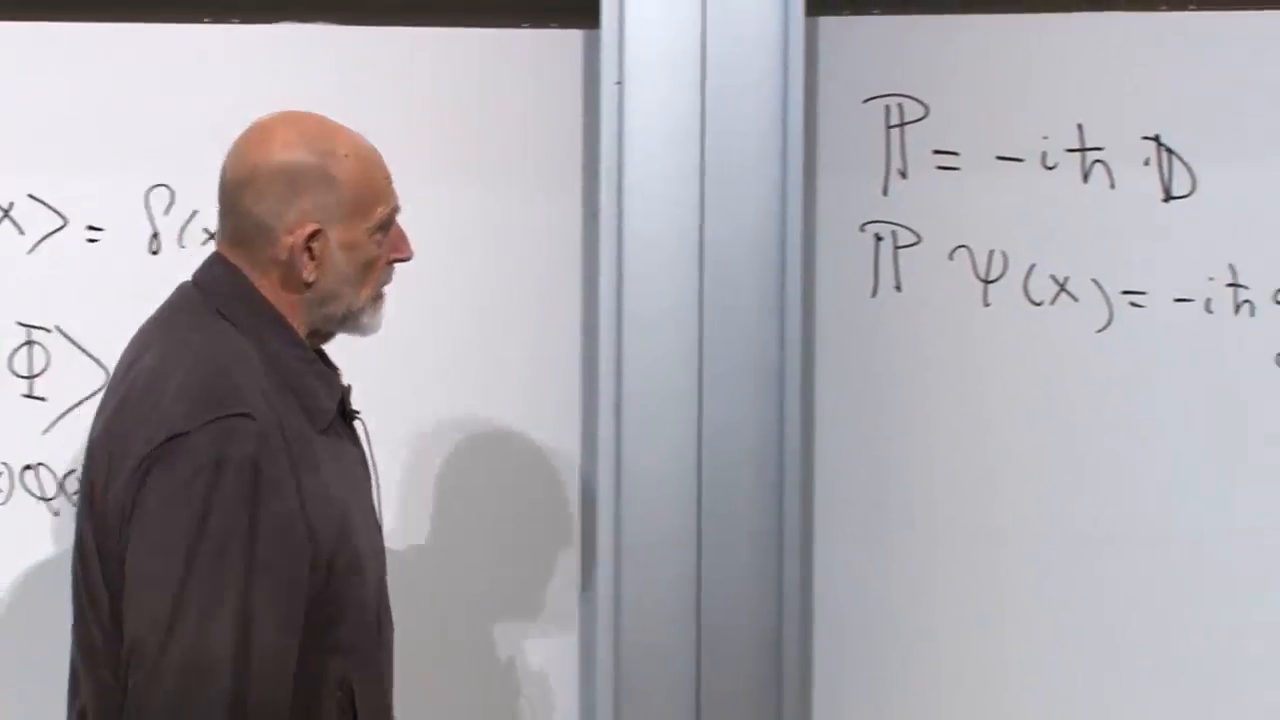
\includegraphics[width=0.88\textwidth]{lecture_09_figure_05.png}
\caption{Произвольное состояние, разложенное по непрерывному базису положений; коэффициент восстанавливается проецированием на \(\ket{x}\).}
\lectureframe{00:35:30}
\end{figure}

Правило Борна задаёт плотность вероятности
\begin{equation}
\rho(x)=|\psi(x)|^2.
\end{equation}
Вероятность на конечном интервале равна
\begin{equation}
P(a<x<b)=\int_a^b|\psi(x)|^2\,dx,
\end{equation}
Нормированное физическое состояние удовлетворяет условию
\begin{equation}
\int_{-\infty}^{\infty}|\psi(x)|^2\,dx=1.
\label{eq:l9-position-normalization}
\end{equation}
Непрерывная ортогональность выражается как
\begin{equation}
\braket{x'}{x}=\delta(x-x').
\label{eq:l9-position-delta}
\end{equation}
Для двух произвольных состояний скалярное произведение принимает вид
\begin{equation}
\braket{\Psi}{\Phi}
=
\int_{-\infty}^{\infty}
dx\,\psi^*(x)\phi(x).
\label{eq:l9-position-inner-product}
\end{equation}

\begin{figure}[htbp]
\centering
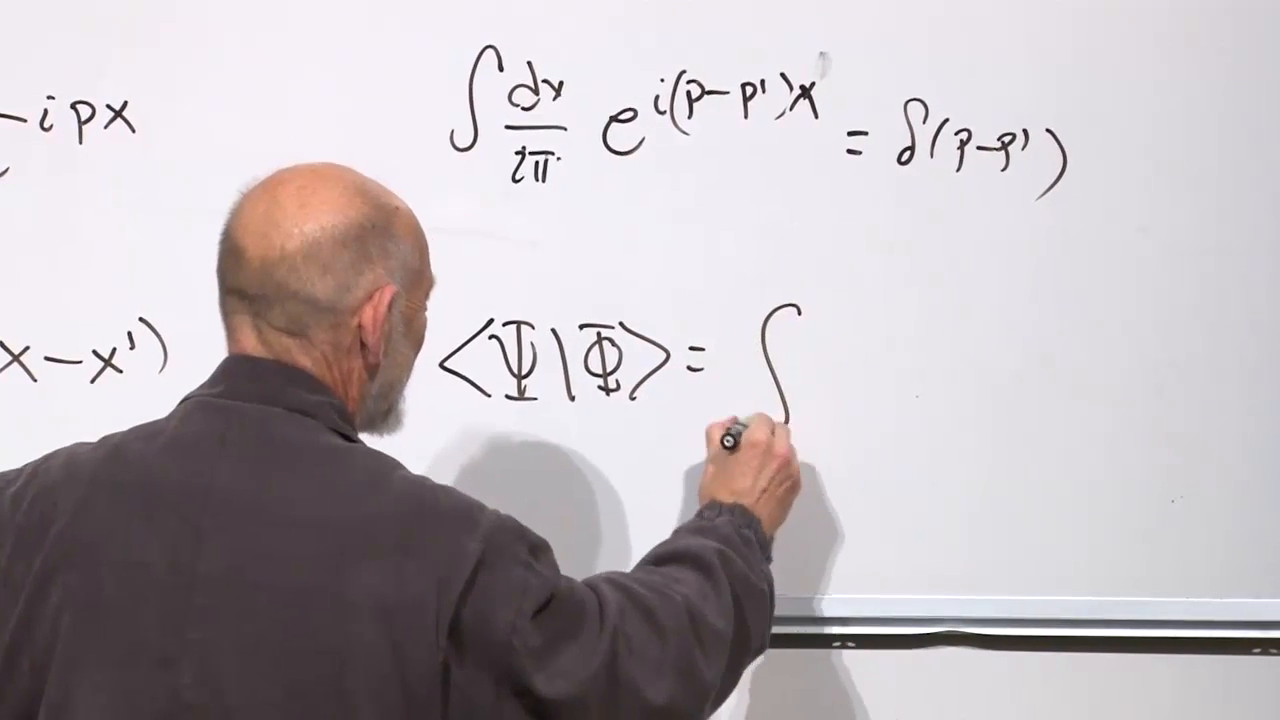
\includegraphics[width=0.88\textwidth]{lecture_09_figure_06.png}
\caption{Нормировка непрерывного базиса и скалярное произведение волновых функций, записанное в координатном представлении.}
\lectureframe{00:41:20}
\end{figure}

\begin{classroomqa}
\audiencequestion{Почему одной координаты достаточно? Не было бы ли избыточным добавление импульса или почти любой другой переменной?}
\lecturerresponse{Для одной частицы в одном измерении функция \(\psi(x)\) целиком задаёт состояние, так что одновременное точное значение \(p\) давало бы слишком много информации. Импульс задаёт другой полный базис, а не дополнительную метку, приписанную каждому \(\ket{x}\). В большем числе измерений совместимую информацию можно комбинировать: например, \(X\) и \(P_y\) коммутируют и могут служить метками совместного базиса. Ограничение относится к некоммутирующим парам, а не просто к числу символов.}
\end{classroomqa}

\begin{classroomqa}
\audiencequestion{Может ли импульс тоже задавать полный базис, и можно ли выразить разложение по нему через положение?}
\lecturerresponse{Да. Базис импульса полон, и его коэффициенты связаны с коэффициентами в базисе положений преобразованием Фурье. Эта связь — центральная конструкция данной лекции.}
\end{classroomqa}

\section{Координата в координатном представлении}

Абстрактный оператор действует на векторы состояния. После выбора базиса то же действие становится конкретной операцией над волновыми функциями. В координатном представлении оператор координаты \(X\) действует умножением:
\begin{equation}
(X\psi)(x)=x\psi(x).
\label{eq:l9-position-operator}
\end{equation}

Состояние, локализованное в \(x_0\), представляется обобщённой волновой функцией \(\delta(x-x_0)\). Применяя \(X\), получаем
\begin{align}
X\delta(x-x_0)
&=
x\delta(x-x_0) \notag\\
&=
x_0\delta(x-x_0),
\label{eq:l9-position-eigenfunction}
\end{align}
где использовалось соотношение~\eqref{eq:l9-delta-multiplication}. Следовательно, \(\delta(x-x_0)\) является собственной функцией \(X\) с собственным значением \(x_0\).

\begin{figure}[htbp]
\centering
\includegraphics[width=0.88\textwidth]{lecture_09_figure_07.png}
\caption{Умножение на \(x\) переводит состояние, локализованное дельта-функцией, в него же, умноженное на \(x_0\), что доказывает, что оно является собственной функцией оператора координаты.}
\lectureframe{00:45:50}
\end{figure}

Ни \(\ket{x_0}\), ни представляющая его дельта-функция не нормированы на единицу в обычном квадратно-интегрируемом смысле. Они дельта-нормированы. Физические локализованные состояния представляют собой конечные волновые пакеты, тогда как точные собственные состояния служат обобщёнными базисными векторами.

\section{Собственные функции импульса}

На предыдущей лекции было показано, что дифференцирование антиэрмитово, а умножение на \(-i\) делает его эрмитовым. Восстанавливая единицы, определим
\begin{equation}
P=-i\hbar\frac{d}{dx},
\qquad
(P\psi)(x)
=
-i\hbar\frac{d\psi}{dx}.
\label{eq:l9-momentum-operator}
\end{equation}
Это корректная наблюдаемая на подходящей области определения. Её отождествление с физическим импульсом будет проверено через её спектр, длину волны и роль в динамике.

Для собственного значения импульса \(p\) решим
\begin{equation}
P\psi_p=p\psi_p,
\end{equation}
или
\begin{equation}
-i\hbar\frac{d\psi_p}{dx}=p\psi_p.
\end{equation}
Решение имеет вид
\begin{equation}
\psi_p(x)=A e^{ipx/\hbar}.
\label{eq:l9-momentum-eigenfunction}
\end{equation}

\begin{figure}[htbp]
\centering
\includegraphics[width=0.88\textwidth]{lecture_09_figure_08.png}
\caption{Представитель в координатном представлении состояния с определённым импульсом — плоская волна \(e^{ipx/\hbar}\).}
\lectureframe{00:51:45}
\end{figure}

Длина волны \(\lambda\) — это смещение, при котором фаза возрастает на \(2\pi\):
\begin{equation}
\frac{p\lambda}{\hbar}=2\pi,
\qquad
\lambda=\frac{2\pi\hbar}{p}.
\label{eq:l9-de-broglie}
\end{equation}
Следовательно, большему импульсу соответствует меньшая длина волны.

Дельта-нормировка фиксирует константу:
\begin{equation}
\psi_p(x)
=
\frac{1}{\sqrt{2\pi\hbar}}e^{ipx/\hbar}.
\label{eq:l9-normalized-momentum-eigenfunction}
\end{equation}
В самом деле,
\begin{align}
\braket{p'}{p}
&=
\int_{-\infty}^{\infty}
dx\,
\psi_{p'}^*(x)\psi_p(x) \notag\\
&=
\int_{-\infty}^{\infty}
\frac{dx}{2\pi\hbar}
e^{i(p-p')x/\hbar} \notag\\
&=
\delta(p-p').
\label{eq:l9-momentum-normalization}
\end{align}
После выбора единиц с \(\hbar=1\) эти формулы принимают вид
\begin{equation}
\psi_p(x)=\frac{1}{\sqrt{2\pi}}e^{ipx},
\qquad
\int\frac{dx}{2\pi}e^{i(p-p')x}
=\delta(p-p').
\end{equation}

\begin{classroomqa}
\audiencequestion{Как можно объявить осциллирующий интеграл равным нулю при \(p\neq p'\), если он не сходится в обычном смысле?}
\lecturerresponse{В лекции используется контролируемый обходной приём. Систему помещают на конечный периодический интервал. Тогда допустимые импульсы образуют дискретное множество, экспоненты ортогональны в обычном смысле, и всякая нормировка конечна. Лишь после этого вычисления интервал следует устремить к бесконечности, превращая дельту Кронекера в дельта-функцию Дирака.}
\end{classroomqa}

\begin{classroomqa}
\audiencequestion{Затрагивает ли тот же вопрос сходимости и вывод дельта-функции через преобразование Фурье?}
\lecturerresponse{Да. Перестановка интегралов там была формальной по той же причине. Вывод для конечного ящика или язык распределений восполняют недостающую строгость. Этот обходной приём допустим, потому что регуляризованное вычисление имеет указанный предел непрерывного случая.}
\end{classroomqa}

\section{Импульсное представление}

Не следует путать два объекта. Функция \(\psi_p(x)\) в уравнении~\eqref{eq:l9-normalized-momentum-eigenfunction} — это представитель в координатном представлении конкретного собственного состояния \(\ket{p}\). Напротив, волновая функция в импульсном представлении произвольного состояния \(\ket{\Psi}\) есть
\begin{equation}
\widetilde{\psi}(p)=\braket{p}{\Psi}.
\label{eq:l9-momentum-wavefunction}
\end{equation}
Подставим волновые функции в координатном представлении для \(\bra{p}\) и \(\ket{\Psi}\):
\begin{align}
\widetilde{\psi}(p)
&=
\int_{-\infty}^{\infty}
dx\,
\braket{p}{x}\braket{x}{\Psi} \notag\\
&=
\int_{-\infty}^{\infty}
\frac{dx}{\sqrt{2\pi\hbar}}\,
e^{-ipx/\hbar}\psi(x).
\label{eq:l9-position-to-momentum}
\end{align}
Это в точности преобразование Фурье. Обратно,
\begin{equation}
\psi(x)
=
\int_{-\infty}^{\infty}
\frac{dp}{\sqrt{2\pi\hbar}}\,
\widetilde{\psi}(p)e^{ipx/\hbar}.
\label{eq:l9-momentum-to-position}
\end{equation}

\begin{figure}[htbp]
\centering
\includegraphics[width=0.88\textwidth]{lecture_09_figure_09.png}
\caption{Проецирование на \(\ket{p}\) превращает волновую функцию в координатном представлении в её преобразование Фурье \(\widetilde{\psi}(p)\).}
\lectureframe{01:05:50}
\end{figure}

Плотность вероятности измерить импульс \(p\) равна
\begin{equation}
\widetilde{\rho}(p)
=
|\widetilde{\psi}(p)|^2,
\qquad
\int_{-\infty}^{\infty}
|\widetilde{\psi}(p)|^2\,dp=1.
\end{equation}
Таким образом, одна волновая функция в координатном представлении содержит достаточно информации, чтобы предсказывать как измерения координаты, так и измерения импульса. Чтобы получить вероятности импульса, нужно выполнить преобразование Фурье функции \(\psi(x)\) и возвести модуль результата в квадрат.

В импульсном представлении роли меняются местами:
\begin{equation}
(P\widetilde{\psi})(p)
=
p\widetilde{\psi}(p),
\qquad
(X\widetilde{\psi})(p)
=
i\hbar\frac{d\widetilde{\psi}}{dp}.
\label{eq:l9-operators-in-p}
\end{equation}
Разность знаков по сравнению с \(P=-i\hbar\,d/dx\) следует из противоположных знаков в паре преобразований Фурье.

\begin{classroomqa}
\audiencequestion{Является ли время оператором, сопряжённым энергии, в том же смысле, в каком координата сопряжена импульсу?}
\lecturerresponse{Время обычно рассматривается как внешний параметр, обозначающий эволюцию состояния, а не как универсальный самосопряжённый оператор в гильбертовом пространстве системы. У реальных часов действительно есть наблюдаемые показания, и улучшение временного разрешения часов имеет энергетические последствия, но соотношение время–энергия требует большей осторожности, чем пара координата–импульс, и здесь не рассматривается.}
\end{classroomqa}

\begin{classroomqa}
\audiencequestion{Какие ещё сопряжённые пары встречаются?}
\lecturerresponse{Важный пример дают угол и соответствующий угловой момент, с оговорками глобального характера, поскольку угол периодичен. В теории поля сопряжёнными являются поле и его канонический импульс. Температура и давление — термодинамические переменные, а не каноническая квантовая пара. Общий принцип задаётся каноническими переменными и их коммутаторами, а не произвольной парой измеримых величин.}
\end{classroomqa}

\begin{classroomqa}
\audiencequestion{В дискретной теории операторы действовали на кеты, а волновые функции лишь перечисляли коэффициенты. Изменилось ли это в непрерывной теории?}
\lecturerresponse{Нет. Волновая функция — это координатный столбец абстрактного кета в выбранном базисе. Матрица, действующая на конечный столбец, и дифференциальный или интегральный оператор, действующий на функцию, — два конкретных представления одной и той же абстрактной операции. Непрерывная метка меняет обозначения, а не логику.}
\end{classroomqa}

\subsection{Неопределённость как факт Фурье}

Состояние с определённым импульсом полностью делокализовано:
\begin{equation}
|\psi_p(x)|^2=\text{constant}.
\end{equation}
Его импульс точен, но положение равномерно распределено по всей прямой. В более общем случае обе функции, связанные преобразованием Фурье, не могут быть узкими одновременно. Сосредоточение \(\widetilde{\psi}(p)\) в узком диапазоне импульсов вынуждает \(\psi(x)\) простираться по большой области, а локализация \(\psi(x)\) требует широкого диапазона импульсов.

В этой лекции количественное неравенство пока не выводится
\begin{equation}
\Delta X\,\Delta P\geq\frac{\hbar}{2}.
\end{equation}
Пока здесь важен структурный момент: принцип неопределённости уже закодирован во взаимно-обратной геометрии преобразований Фурье. Это непрерывный аналог перехода между несовместимыми спиновыми базисами.

\section{Гамильтониан порождает эволюцию во времени}

Гамильтониан \(H\) эрмитов, представляет энергию и порождает унитарную эволюцию во времени. Зависящее от времени уравнение Schr\"odinger имеет вид
\begin{equation}
i\hbar\frac{d}{dt}\ket{\Psi(t)}
=
H\ket{\Psi(t)}.
\label{eq:l9-abstract-schrodinger}
\end{equation}
В координатном представлении
\begin{equation}
i\hbar\frac{\partial\psi(x,t)}{\partial t}
=
H\psi(x,t),
\label{eq:l9-position-schrodinger}
\end{equation}
где правая часть означает выбранное координатное представление действия гамильтониана на функцию.

\subsection{Намеренно простой линейный гамильтониан}

Рассмотрим
\begin{equation}
H=cP.
\label{eq:l9-linear-hamiltonian}
\end{equation}
Это не обычный нерелятивистский гамильтониан свободной частицы. Он выбран потому, что каждый шаг можно проследить непосредственно.

\begin{figure}[htbp]
\centering
\includegraphics[width=0.88\textwidth]{lecture_09_figure_10.png}
\caption{Уравнение Schr\"odinger и линейный гамильтониан \(H=cP\), выбранный в качестве простейшего примера эволюции частицы.}
\lectureframe{01:17:45}
\end{figure}

Используя \(P=-i\hbar\,\partial_x\),
\begin{align}
i\hbar\frac{\partial\psi}{\partial t}
&=
c\left(-i\hbar\frac{\partial}{\partial x}\right)\psi, \notag\\
\frac{\partial\psi}{\partial t}
&=
-c\frac{\partial\psi}{\partial x},
\end{align}
или
\begin{equation}
\frac{\partial\psi}{\partial t}
+c\frac{\partial\psi}{\partial x}=0.
\label{eq:l9-transport-equation}
\end{equation}

\begin{figure}[htbp]
\centering
\includegraphics[width=0.88\textwidth]{lecture_09_figure_11.png}
\caption{Линейный гамильтониан сводит уравнение Schr\"odinger к уравнению переноса первого порядка.}
\lectureframe{01:20:05}
\end{figure}

Общее решение имеет вид
\begin{equation}
\psi(x,t)=f(x-ct),
\label{eq:l9-rigid-translation}
\end{equation}
для любого нормируемого начального профиля \(f\). При \(t=0\) профиль равен \(f(x)\). В более поздние моменты времени все особенности профиля смещаются вправо на \(ct\). Комплексная волновая функция, её действительная и мнимая части, а также плотность вероятности сохраняют свою форму:
\begin{equation}
|\psi(x,t)|^2=|f(x-ct)|^2.
\end{equation}
Следовательно,
\begin{equation}
\expect{X}_t=\expect{X}_0+ct.
\end{equation}

Символ \(c\) был выбран так, чтобы напоминать о скорости света. Модель похожа на одиночное одномерное хиральное безмассовое возбуждение: каждая допустимая компонента движется в одном направлении с одной и той же скоростью. Это не полная теория фотона. Низкоэнергетические одномерные фононы с фиксированной скоростью звука дают другую аналогию. Поскольку \(E=cp\), допущение обоих знаков \(p\) также допускает отрицательные энергии — ещё один признак того, что это намеренно ограниченная учебная модель.

\begin{classroomqa}
\audiencequestion{Описывало бы \(H=cP\) какую-либо свободную частицу, если бы \(c\) заменили на скорость этой частицы?}
\lecturerresponse{Нет. Фиксированный коэффициент в \(H=cP\) означает, что все импульсные компоненты имеют одну и ту же скорость. Для нерелятивистской частицы скорость равна \(p/m\), так что она зависит от импульса. Запись \(vP\) при \(v=p/m\) уже не линейна по \(P\); она указывает на квадратичный гамильтониан.}
\end{classroomqa}

\begin{classroomqa}
\audiencequestion{Не должна ли волновая функция обычного свободно движущегося электрона просто жёстко сдвигаться?}
\lecturerresponse{Только очень специальное дисперсионное соотношение приводит к жёсткому переносу любого профиля. Обычный пакет свободного электрона содержит много импульсных компонент, фазы которых эволюционируют с разными скоростями. Его центр движется, но его форма, вообще говоря, расплывается.}
\end{classroomqa}

\subsection{Сравнение с классическим случаем}

Для классического гамильтониана \(H=cp\) уравнения Гамильтона дают
\begin{equation}
\dot{x}=\frac{\partial H}{\partial p}=c,
\qquad
\dot{p}=-\frac{\partial H}{\partial x}=0.
\label{eq:l9-linear-hamilton-equations}
\end{equation}

\begin{figure}[htbp]
\centering
\includegraphics[width=0.88\textwidth]{lecture_09_figure_12.png}
\caption{Уравнения Гамильтона для \(H=cp\): постоянная скорость вправо и сохранение импульса.}
\lectureframe{01:25:20}
\end{figure}

Квантовое распределение вероятности и его среднее значение подчиняются тому же простому движению. Это совпадение — первое конкретное напоминание о том, что квантовая эволюция, построенная из классического гамильтониана, должна в надлежащем смысле воспроизводить классические уравнения.

\section{Нерелятивистская свободная частица}

Для обычной частицы массы \(m\) при отсутствии силы классическая кинетическая энергия равна
\begin{equation}
H=\frac{p^2}{2m}.
\end{equation}
Квадратичная форма симметрично трактует \(p\) и \(-p\), поэтому частицы, движущиеся влево и вправо, имеют одну и ту же положительную энергию. Квантование заменяет \(p\) оператором \(P\):
\begin{equation}
H=\frac{P^2}{2m}.
\label{eq:l9-free-hamiltonian}
\end{equation}
Подставим \(P=-i\hbar\,\partial_x\) в уравнение Schr\"odinger:
\begin{align}
i\hbar\frac{\partial\psi}{\partial t}
&=
\frac{1}{2m}
\left(-i\hbar\frac{\partial}{\partial x}\right)^2
\psi \notag\\
&=
-\frac{\hbar^2}{2m}
\frac{\partial^2\psi}{\partial x^2}.
\label{eq:l9-free-schrodinger}
\end{align}

\begin{figure}[htbp]
\centering
\includegraphics[width=0.88\textwidth]{lecture_09_figure_13.png}
\caption{Уравнение Schr\"odinger для свободной частицы, полученное из \(H=P^2/(2m)\) и \(P=-i\hbar\,\partial_x\).}
\lectureframe{01:33:50}
\end{figure}

Плосковолновая компонента с импульсом \(p\) имеет энергию
\begin{equation}
E(p)=\frac{p^2}{2m}.
\end{equation}
В отличие от линейного случая \(E=cp\), наклон этого дисперсионного соотношения зависит от \(p\):
\begin{equation}
v_{\mathrm{group}}
=
\frac{dE}{dp}
=
\frac{p}{m}.
\end{equation}
Поэтому различные импульсные компоненты локализованного пакета движутся с разными групповыми скоростями. Их относительные фазы меняются, компоненты расходятся, и пакет расплывается. Решающее различие состоит в том, что \(H=cP\) жёстко переносит любой профиль, тогда как \(H=P^2/(2m)\) приводит к дисперсионному движению свободной частицы.

\section{Что было установлено}

Математическое отступление не было отделено от физики. Плоские волны и дельта-функция Дирака сформировали аппарат непрерывных базисов. Оператор положения действует умножением, оператор импульса действует дифференцированием, а собственные состояния импульса являются плоскими волнами. Проецирование произвольного состояния на эти собственные состояния даёт преобразование Фурье его координатной волновой функции. Поэтому положение и импульс — это два альтернативных представления одного состояния, а их неопределённость — это знакомая взаимно обратная ширина пары Фурье.

Тот же аппарат представлений затем превращает гамильтониан в дифференциальное уравнение. Линейная функция импульса порождает жёсткий перенос; квадратичная кинетическая энергия порождает уравнение Schr\"odinger для свободной частицы и дисперсию. Курс перешёл от основ измерения к механике движения, не меняя своего центрального языка: состояния, базисы, эрмитовы наблюдаемые, амплитуды и унитарная эволюция.
